\subsection{L'inizio: trasmutazioni nucleari}
Le osservazione di Bequerel della presenza di trasmutazioni di atomi e la radiazione emessa durante questo processo è dell'ordine del $MeV$ di differente \textbf{carica} e \textbf{grado di penetrazione}. Questa energia per atomo + $10^6$ volte maggiore delle reazioni chimiche. Oltre a questo si osserva che a differenza delle reazioni chimiche c'è un cambio di natura degli stessi atomi.

L'esperimento di Rutherford dimostra che la carica positiva dell'atomo è concentrata in un nucleo ed è da qui che parte la fisica nucleare anche se paradossalmente la fisica delle particelle elementari (subnucleare) inizia prima con la scoperta dell'elettrone.

Sappiamo che le dimensioni del nucleo sono molto minori rispetto alle dimensioni atomiche ($10^{-10}\,m$). Gli elettroni occupano lo spazio restante, ma costituiscono una frazione piccola della massa atomica, infatti:
\begin{equation*}
    m_e=9.10938291\times10^{-31}\,kg \,<<M_{\text{atomi}}\,10^{-27}-10^{-25}\,kg
\end{equation*}
Le dimensioni dei nuclei sono stimabili da considerazioni quantistiche (ci sono anche delle misure dirette, ad esempio, attraverso gli esperimenti di Hofstadter). La determinazione sperimentale delle masse di nuclei permette di formulare le basi della struttura nucleare: \textbf{nuclei sono costituiti da protoni e neutroni} $m_p$ e $m_n$ che hanno circa la stessa massa. Questo ci porta a spiegare perchè la massa atomica per molti elementi è \textbf{quasi} un multiplo intero. Quasi perchè la massa nucleare è minore di quella dei costituenti. Prima osservazione diretta in cui si tocca con mano l'equivalenza tra massa ed energia. Lo studio dell'energia di legame fornisce importanti informazioni qualitative sulle interazioni nucleari: \textbf{modello a goccia}.
\subsection{Sistema di unità naturali e costanti fondamentali}
Prima di inziare la discussione sulle masse e dimensioni dei nuclei consideriamo due costanti fondamentali della natura: la \textbf{relatività ristretta} introduce come costante la \textbf{velocità della luce nel vuoto}: $c=2.99792458\times10^8\,m/s$. Questa costante ci permette di collegare tra di loro unità di misura di grandezze diverse. Posso:
\begin{itemize}
    \item massa $[M]$ $\,\Leftrightarrow\,$ momento $[P]=[Mc]\,\Leftrightarrow\,$ energia $[E]=[Mc^2]$
    \item lunghezza $[L]$ $\,\Leftrightarrow\,$ tempo $[T]=[L/c]$
\end{itemize}
La \textbf{meccanica quantistica} introduce la \textbf{costante di Plank}, come unità fondamentale dell'azione (area nello spazio delle fasi): $\hbar=\frac{h}{2\pi}=1.054571726\times10^{-34}\,Js$. Questa costante, come con la costante velocità della luce, ci permette di collegare tra di loro unità di misura di grandezze diverse. Posso:
\begin{itemize}
    \item energia $[E]$ $\,\Leftrightarrow\,$ tempo $[T]=[\hbar/E]$
    \item lunghezza $[L]$ $\,\Leftrightarrow\,$ momento $[P]=[\hbar/L]$
\end{itemize}
In pratica possiamo definire una sola unità di misura fondamentale e tutte le altre possono venire derivate da questa attraverso $\hbar$ e $c$. Un sistema che useremo spesso durante il corso è: 
\begin{itemize}
    \item \textbf{unità di misura dell'energia:} $eV$;
    \item unità di misura della massa: $eV/c^2$;
    \item unità di misura della quantità di moto: $eV/c$;
    \item unità di misura del tempo: $eV^{-1}\hbar$;
    \item unità di misura della lunghezza: $eV^{-1}\hbar c$;
    \item \textbf{unità di misura della velocità:} $c$;
    \item \textbf{unità di misura del momento angolare:} $\hbar$.
\end{itemize}
Numericamente è come usare un sistema di unità in cui:
\begin{equation*}
    \hbar=c=1
\end{equation*}
Questo sistema in cui $\hbar=c=1$ viene spesso chiamato sistema naturale. Calcoli e formule sono spesso molto semplificati in un sistema naturale. Per trasformare i risultati in unità SI si tratta di moltiplicarri per i corretti fattori di conversione.
\begin{equation*}
    c\approx 3\times10^{8}\,m/s \qquad \hbar \approx \frac{2}{3}\times10^{-21}\,MeVs \qquad \hbar c \approx 200\, MeVfm
\end{equation*}
Dove $fm$ indica il fermi: $1\,fm=1\times 10^{-15}\,m$
\subsection{Costante di struttura fine}
La quantità che compare nell'energia potenziale elettrostatica: 
\begin{equation*}
    \frac{e^2}{\varepsilon_0}=\frac{(1.602176565\times10^{-19}\,C)^2}{8.854187817\times10^{-12}\,F/m}=2.899158908\times10^{-27}Jm=18.09512739\,MeVfm
\end{equation*}
Ha le dimensioni di Energia $\times$ Lunghezza = [$\hbar c$]. Il suo valore in sistema di unità naturali è:
\begin{equation*}
    \frac{e^2}{\varepsilon_0\hbar c}=0.09170123392
\end{equation*}
è quindi indipendente dall'unità fondamentale scelta. In questi sistemi la carica elettrica elementare è un numero adimensionale:
\begin{equation*}
    \sqrt{\frac{e^2}{\varepsilon_0\hbar c}}=0.3028221209
\end{equation*}
Il coefficiente che compare in molte espressioni dell'elettromagnetismo:
\begin{equation*}
    \frac{e^2}{4\pi\varepsilon_0}\frac{1}{\hbar c}=\alpha=\frac{1}{137.035999074}
\end{equation*}
Prende il nome di \textbf{costante di struttura fine}. Ad esempio, la sezione d'urto di Rutherford diventa ora:
\begin{equation*}
    \frac{d\sigma}{d\Omega}=\left(\frac{ZZ_\alpha}{e}\alpha\right)^2\frac{1}{\sin^4{\theta/2}}\left(\frac{\hbar c}{E}\right)^2
\end{equation*}
Si nota come il termine $\hbar c/E$ è una lunghezza.
\subsection{Dimensioni dei nuclei}
Nell'esperimento di Rutherford non si riusciva a distinguere la dimensione del nucleo. Una prima stima può avvenire dai decadimenti $\alpha$. Se prendiamo un'energia tipica dei decadimenti $\alpha$: $T_\alpha=5\,MeV$, questo corrisponde ad un momento: $p_\alpha=\sqrt{2m_\alpha T_\alpha}\approx 200\,MeV$. Assumiamo che la particella $\alpha$ sia inizialmente confinata nel nucleo. Quando è confinata il suo momento varia di $\pm p_\alpha$ rimbalzando all'interno del nucleo. Quindi:$\Delta p = 2p_\alpha$. Dal principio di indeterminazione: $\Delta x\Delta p\approx 1$ (nel sistema di unità naturali, infatti $\Delta x\Delta p\le\frac{\hbar}{2}$):
\begin{equation*}
    \Delta x \approx \frac{1}{\Delta p}\approx 0.0025\,MeV^{-1} \approx 0.5\,fm
\end{equation*}
Con questo ragionamento si è arrivati a stimare l'ordine di grandezza del nucleo della particella $\alpha$. Questa dimensione ha anche senso con quello che ci si aspettava in quanto, come abbiamo detto il nucleo è molto più piccolo rispetto all'atomo. Infatti un atomo ha un raggio dell'ordine di grandezza di $\sim10^{-10}\, m$ mentre il nucleo $\sim10^{-15}\,m$. Una misura sistematica si ottiene dallo studio della sezione d'urto elettrone-nucleo: se il parametro d'impatto è minore delle dimensione nucleare la sezione d'urto differisce della sezione d'urto coulombiana. Si ottiene: 
\begin{equation*}
    R\sim r_0A^{1/3}\qquad r_0=1.2\,fm 
\end{equation*}
Questo è un risultato fenomenologico molto importante. Una cosa particolare che si nota subito è che il volume è direttamente proporzionale al peso atomico $A$.
\subsection{Classificazione dei nuclei}
I nuclei sono costituiti da \textbf{protoni} e \textbf{neutroni}. La carica del nucleo è data dal numero di protoni: il numero atomico $Z$ che determina le proprietà chimiche dell'atomo risultante ed è di solito indicato attraverso il simbolo dell'elemento chimico. La massa del nucleo dipende principalmente dal numero di nucleoni: è indicato dal numero di massa $A$ che è dato dalla somma di $Z$ e dal numero di neutroni $N$. Ad esempio:
\begin{equation*}
    \ch{^9Be} \text{  berilio con } A=9 \text{ e } Z=4
\end{equation*}
Da cui è facile ricavare il numero di neutroni $N=A-Z=5$. Se fosse necessario indicare esplicitamente $Z$ è possibile anche la notazione: $\ch{^A_ZX}$.

Nuclei con lo stesso $Z$ ma diverso $N$ sono detti \textbf{isotopi} dello stesso elemento. Nuclei con lo stesso $A$, ma diverso $Z$ sono detti \textbf{isobari}. Nuclei con lo stesso $N$, ma diverso $Z$ sono detti \textbf{isotoni}. Un nucleo con determinati valori di $A$ e $Z$ può trovarsi in stati eccitati, \textbf{isomeri} o \textbf{risonanze}, da cui solitamente decade nello stato fondamentale emettendo radiazione elettromagnetica (raggi $\gamma$).
\subsection{Carta dei nuclidi}
Questa è la mappa che rappresenta tutti i nuclei che si sono riusciti ad osservare. La zona centrale è costituita dai nuclei stabili dopodichè abbiamo il punto più alto raggiunto dal bismuto che è ancora classificabile stabile anche se ha una vità media di $10^{19}\,yr$. Tenendo conto che l'universo ha una decina di miliardi di anni è più che giusto farlo.
%IMMAGINE nuclidi
\begin{figure}[htp!]
  \centering
  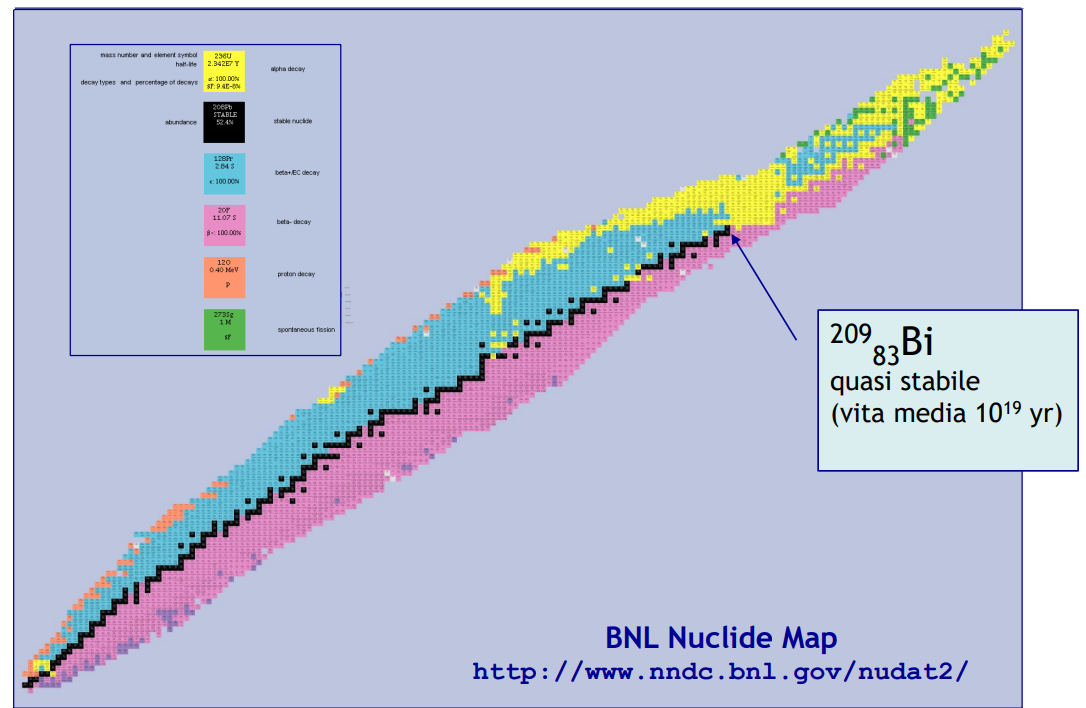
\includegraphics[scale=0.6]{Lezione2/nuclidi.png} 
\end{figure}
\subsection{Masse dei nuclei}
Come abbiamo accennato in precedenza la massa di un nucleo è inferiore alla somma delle masse dei costituenti:
\begin{equation*}
    M(A,Z)< Zm_p+(A-Z)m_n
\end{equation*}
Dove: $m_p=938.27\,MeV/c^2$ e $m_n=939.57\,MeV/c^2$. La differenza di massa è dovuta all'energia di legame (\textbf{binding energy}) dovuta alle forze nucleari:
\begin{equation*}
    \text{B.E.}/c^2=M(A,Z)-Zm_p-(A-Z)m_n
\end{equation*}
\textbf{Il fatto che la massa del sistema sia minore delle sue componenti ne garantisce la stabilità}. Da notare che questa energia è \textbf{negativa}. L'energia potenziale (dovuta dalla presenza di legami) di questi oggetti impedisce al nucleo di frammentarsi, quindi è necessario fornire energia per poter dividere un nucleo. Una quantità fisicamente importante è l'energia media di legame per nucleone:
\begin{equation*}
    \frac{B}{A}=-\frac{\text{B.E.}}{A}=\frac{\left[ Zm_p+(A-Z)m_n-M(A,Z)\right]c^2}{A}
\end{equation*}
Sottointendendo le unità naturali, le masse sono espresse in $MeV$ e quindi tutto diventa: $m_p=938.27\,MeV$ e $m_n=939.57\,MeV$ in quanto $\hbar=c=1$. Dobbiamo però ricordarci che dobbiamo sempre tornare indietro.
\begin{equation*}
    \text{B.E.}=M(A,Z)-Zm_p-(A-Z)m_n
\end{equation*}
\begin{equation*}
    \frac{B}{A}=-\frac{\text{B.E.}}{A}=\frac{\left[ Zm_p+(A-Z)m_n-M(A,Z)\right]}{A}
\end{equation*}
\subsection{Spettrometro di massa}
%IMMAGINE spet ffo
\begin{figure}[htp!]
  \centering
  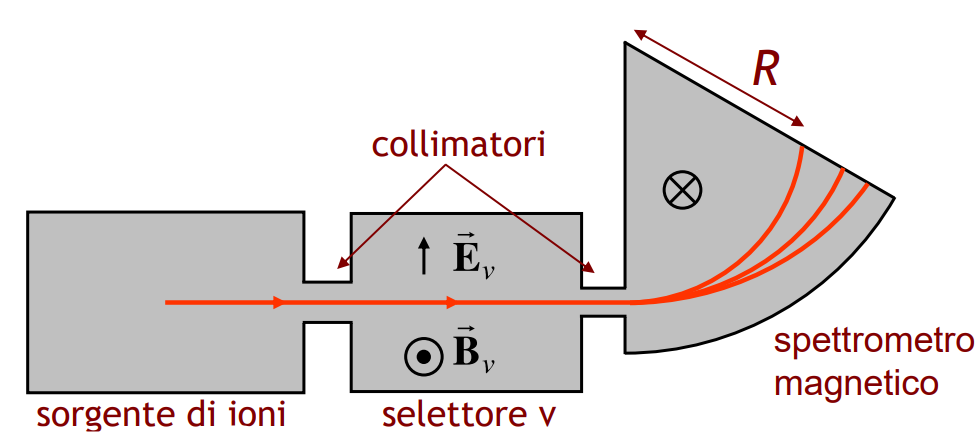
\includegraphics[scale=0.4]{Lezione2/spet.png}
  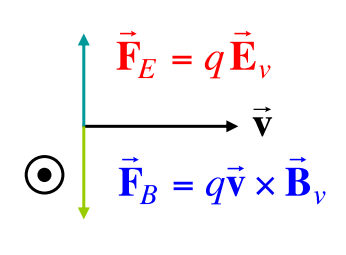
\includegraphics[scale=0.6]{Lezione2/ffo.png} 
\end{figure}
Per la misura di \textbf{masse atomiche} (le masse che misuro non rappresentano la sola massa del nucleo ma è facilmente riconducibile attraverso la massa dell'elettrone) si usano \textbf{spettrometri di massa}. Il principio di funzionamento è il seguente: parto da una sorgente di ioni, non prendo gli atomi ma cerco di produrre degli atomi ionizzati e accellerati. Gli ioni che ho iniziato ad accellerare entrano nel \textbf{selettore di velocità} in cui è presente un campo elettrico e un campo magnetico. Viene definito selettore di velocità perchè solo le particelle che viaggiano in linea retta attraversano i collimatori. I due campi interagiscono con la particella in movimento e applicano due forze. La forza elettrica e la forza magnetica si bilanciano: $\mathbf{F}_E=-\mathbf{F}_B$ quando:
\begin{equation*}
    \mathbf{F}_E=q\mathbf{E}_v \quad \mathbf{F}_B=q\mathbf{v}\times\mathbf{B}_v \,\Rightarrow \, v=\frac{E_v}{B_v}
\end{equation*}
Quindi imponendo un certo valore ai due campi riesco a selezionare solo gli ioni con una certa velocità. Dopo il collimatore gli ioni entrano in uno \textbf{spettrometro magnetico}. Le particelle cariche vengono deviate con una traiettoria circolare:
\begin{equation*}
    qvB=m\frac{v^2}{R} \quad mv=qBR \quad m=q\frac{B_v}{E_v}BR
\end{equation*}
siccome la velocità è uguale per tutte le particelle, se hanno diversa massa hanno un diverso raggio di curvatura. Masse diverse hanno \textbf{raggi diversi}.

C'è un problema: a noi interessano precisioni sulle masse che siano minori $\sim0.1\,MeV$. Se prendo un atomo con $A=100$ e guardo la massa di un questo oggetto, abbiamo visto che circa abbiamo $1000\,MeV$ per ogni nucleone avremo nella misura $100000\,MeV$. Come faccio ad avere una precisione così piccola rispetto alla misura che faccio? Per poter determinare la massa con precisione occorre: misurare con precisione $R$, $E_v$, $B_v$ e $B$ oltre che renderli \textbf{stabili}, \textbf{uniformi} e \textbf{omogenei}. Allora quello che si fa non è tanto misurare la massa di un singolo atomo ma \textbf{rapporti di masse}. In questo modo si ottengono precisioni migliori. Si utilizzano due molecole che hanno \textbf{circa la stessa massa}, ad esempio:
\begin{equation*}
    \ch{^{160}Gd} \,\approx \, \ch{C_12H_16} \qquad A_{\ch{C_12H_16}} =12\times12+16\times1
\end{equation*}
In questo modo si possono utilizzare le \textbf{stesse regolazioni} di $E$ e $B$ per le due molecole. Le molecole passano attraverso le \textbf{stesse regioni} dell'apparato:
\begin{equation*}
    m_1=q\frac{B_v}{E_v}BR_1 \, \,\,\,\ch{^{160}Gd} \qquad m_2=q\frac{B_v}{E_v}BR_2 \,\,\,\,\ch{C_12H_16}
\end{equation*}
In questo modo nel rapporto delle due masse spariscono tutti i contributi non omogenei e non ideali dovuti al campo magnetici ed elettrico presenti nella formula e quindi il rapporto dipende solo dai \textbf{raggi}:
\begin{equation*}
    \frac{m_1}{m_2}=\frac{R_1}{R_2}
\end{equation*}
Il \textbf{carbonio} consente numerose possibilità di realizzare le masse volute. Questo perchè si possono creare tantissime molecole. Normalmente viene tabulato il \textbf{peso atomico}:
\begin{equation*}
    m(A,Z)=M(A,Z)+Zm_e-\frac{B_e(Z)}{c^2}
\end{equation*}
Questo include le masse degli elettroni e la loro piccola energia di legame $B_e$, espresso in \textbf{unified atomic mass unit} ($u$):
\begin{equation*}
    u=\frac{1}{12} \text{della massa di un atomo di }\ch{^{12}C}
\end{equation*}
Quindi:
\begin{equation*}
    1\,u=931.49\,MeV/c^2=1.6605\times10^{-27}\,kg
\end{equation*}
\begin{equation*}
    N_A=6.022142\times10^{23}\,\text{mol}^{-1}\text{ è il numero di atomi contenuti in } 12\,g \text{ di } \ch{^{12}C}
\end{equation*}
Si definisce \textbf{eccesso di massa} la differenza rispetto ad $A\,u$:
\begin{equation*}
    \text{Mass esxcess}=m(A,Z)-Au
\end{equation*}
Questa grandezza è la massa dell'atomo meno $A$ volte l'unità di massa atomica. Questo perchè il grosso della massa dell'atomo è dovuto dal nucleo e quindi pari al numero di nucleoni presenti moltiplicati per $A$. Su questo valor medio si vedono meglio le variazioni di energia di legame che mi fanno aumentare o diminuire la massa di un atomo.
Questo perchè la massa può essere molto grande ma a me interessa l'energia di legame e quindi facendo questa differenza uso numeri più piccola.
Un eccesso di massa negativo vuol dire che il nucleo è molto legato, quindi in una scala lineare più l'eccesso di massa è basso più il mio nucleo è legato.
%IMMAGINE gra
\begin{figure}[htp!]
  \centering
  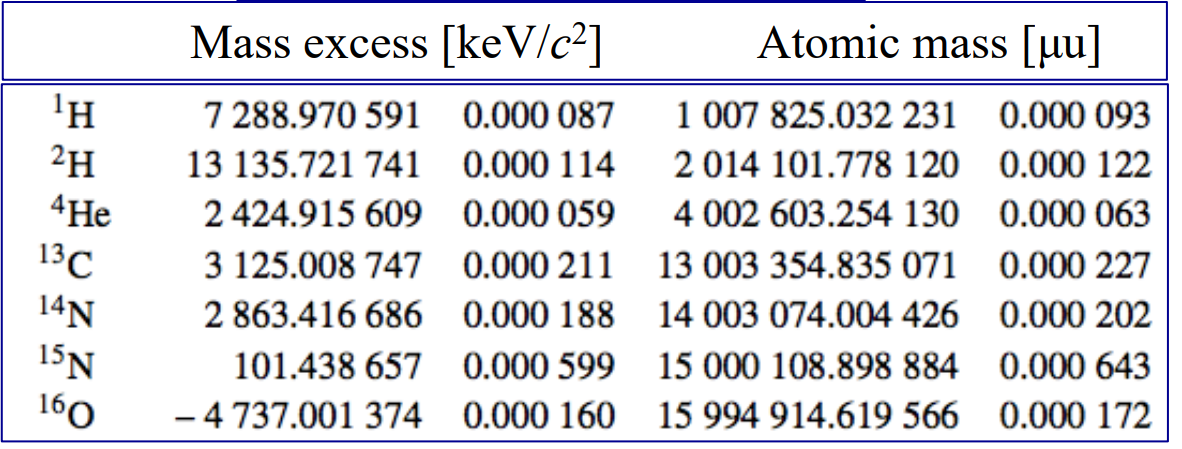
\includegraphics[scale=0.5]{Lezione2/gra.png} 
\end{figure}

Dal grafico si può vedere la massa atomica in $\mu u$ ($10^{-6}\,u$). Le colonne di fianco al valore sono le incertezze. Si vede che a differenza del $\ch{^{12}C}$ l'ossigeno ($\ch{^{16}O}$) è molto più legato e quindi l'eccesso di massa è negativo (infatti la massa atomica è leggermente minore rispetto alla massa dei nucleoni presi singolarmente).
\subsection{Isotopi e pesi atomici}
Uno spettrometro di massa può venire usato come separatore di isotopi, sia come analisi di composizione che come produzione di specifici nuclidi. I pesi atomici degli elementi tengono conto dell'abbondanza isotopica, tipicamente differiscono da $A$ di frazioni di $10^{-3}$ eccetto quando sono presenti diversi isotopi con abbondanza comparabile. Si fa una vera e propria media pesata tra i vari isotopi come peso l'abbondanza in natura dei vari nuclei.
\subsection{Energia di legame per nucleone}
%IMMAGINE el
\begin{figure}[htp!]
  \centering
  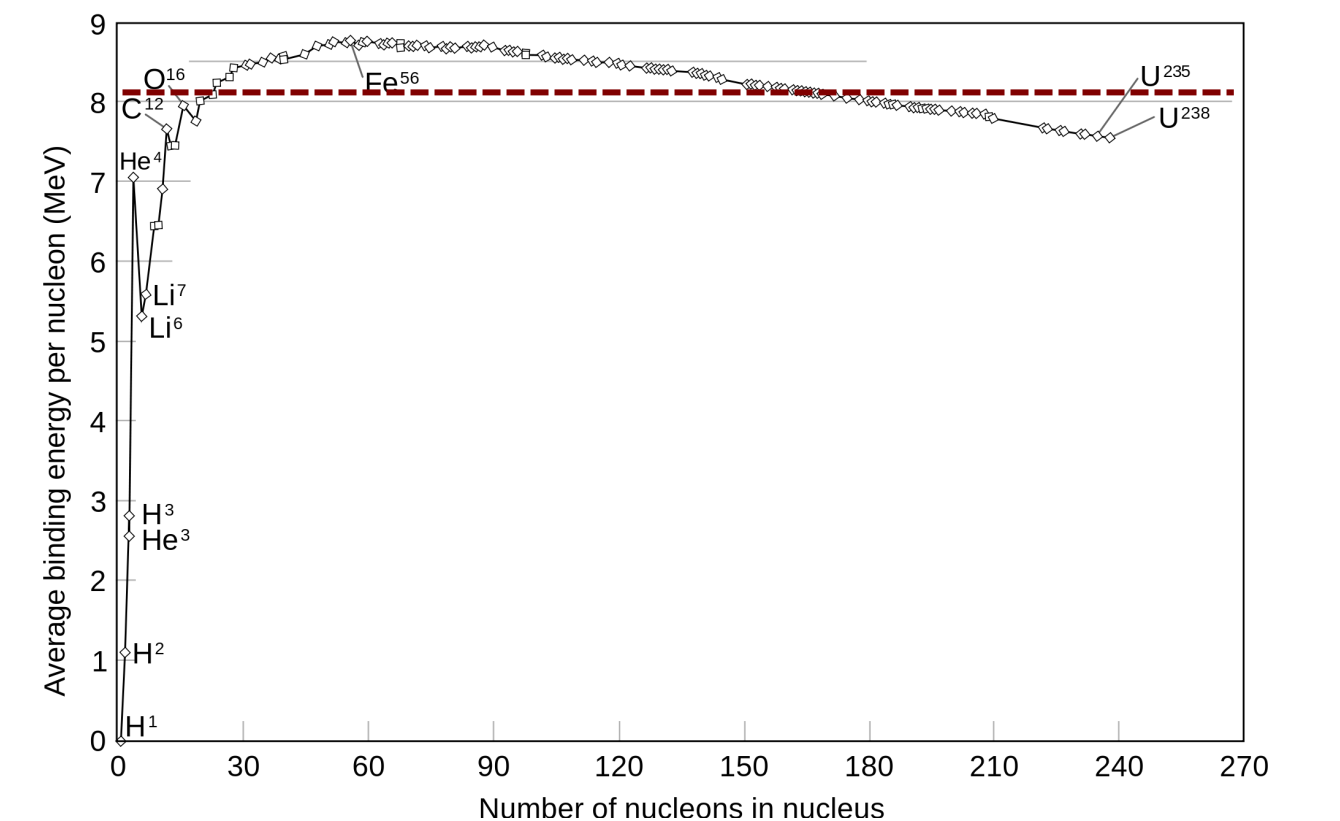
\includegraphics[scale=0.5]{Lezione2/el.png} 
\end{figure}
Abbiamo parlato di energia di legame e di energia di legame per nucleone che non è altro che la B.E. diviso il numero di nucleoni. Ricordo che ci sono delle convenzioni per cui la B.E. è negativa mentre l'energia di legame per nucleone è positiva in quanto cambio il segno.

Se prendiamo un certo numero di massa $A$ e andiamo a vedere per questo numero di massa quale è l'energia di legame del nucleo più stabile posso fare delle considerazioni: la prima cosa è che eccetto per la prima parte (a numeri di massa bassi dove l'energia di legame varia di molto) abbiamo una zona in cui l'energia media di legame è approssimativamente costane: B/A$\sim8\,MeV$ per nucleone. Questa osservazione ci porta a concludere che l'interazione nucleare, cioè l'interazione che lega insieme i diversi nucleoni per costruire i nuclei è un'interazione di breve range, cioè due nucleoni sentono questa forza solo quando sono vicini. Come sono legate le due cose?
\subsection{Interazioni a lungo e corto range}
Mettiamo a confronto le interazione di lungo e corto range per capire cosa lega l'energia di legame per nucleone costante e il numero elevato di $A$:
\begin{itemize}
    \item Interazione a lungo range (es. interazione coulombiana) se abbiamo un inseme di oggetti che forma un aggregato e a questo aggiungiamo una particella, allora questa particella quando arriva interagisce con tutte le altre particelle presenti. Quindi l'energia della particella del sistema $A+1$: $E_{A+1} \propto A$. L'energia totale è proporzionale al numero di coppie: $E\propto A(A-1)/2$. Quindi la mia dipendenza dell'energia totale è grosso modo proporzionale ad $A^2$ e quindi l'energia per nucleone sarà divisa $A$ e quindi proporzionale ad $A$.
    \item Interazione a breve tange (es. legami molecolari) ho che una particella che aggiungo interagisce solo con le particelle più vicine. Quindi l'energia della particella $A+1$: $E_{A+1} \sim $ costante. Essendo una costante ho che l'energia totale è proporzionale ad $A$ $E\propto A$ e quindi se vado a vedere l'energia per nucleone dividendo per $A$ ho che questa energia rimane circa costante.
\end{itemize}
Un'altra cosa che si nota da questo grafico vediamo che c'è un massimo di energia per nucleone. Questo massimo è raggiungo in corrispondenza del $\ch{^{56}Fe}$ e sostanzialmente quello che abbiamo equivale a dire che se prendo dei nuclei con un $A$ minore, sarà energeticamente favorevole (conveniente) combinare nuclei leggeri in un nucleo pesante. Questo è il processo di \textbf{fusione nucleare}. Questo processo spiega come si sono formati i nuclei più leggeri. Infatti la fusione nucleare è presente nel processo di \textbf{nucleosintesi primordiale} e \textbf{stellare}. Al di \textbf{sopra} io ho bisogno di energia per mettere insieme dei nucleoni in quanto l'energia di legame è più bassa per poter costruire questi nuclei devo fornire energia esternamente. Quindi devono venire prodotti da altri meccanismi ad esempio da esplosioni di \textbf{supernove} in cui mi ritrovo ad avere le condizioni energetiche tale da formare effettivamente questi nuclei più pesanti.

Altre informazioni che si possono ottenere dal grafico sono quelle che derivano dalle irregolarità presenti all'inizio del grafico. Infatti l'energia media di legame presenta irregolarità nella regione di basse masse: ad esempio l'elio-4 ($\ch{^4He}$) che è anche la famosa particella $\alpha$ è molto più legato rispetto ai suoi stati adiacenti più o meno pesanti. I modelli nucleari dovranno spiegare queste proprietà. In particolare non vediamo nuclei stabili con $A=5$ e $A=8$. Ad esempio dall'elio-4 si passa direttamente al litio-6 ($\ch{^6Li}$) e non c'è un oggetto con $A=5$. Sono due nuclei che non si riescono a formare in quanto sono in competizione con la formazione di particelle $\alpha$ che sono molto più legate. Questa cosa permette il verificarsi dei \textbf{decadimenti }$\alpha$ di elementi pesanti. Infatti questo tipo di decadimento è il primo che è stato osservato. Il fatto che elementi più pesanti si trasformano in nuclei più leggeri emettendo particelle $\alpha$ permette di risalire la curva di legame e quindi diventa energeticamente possibile.
\subsection{La barriera di massa A=5 e A=8}
%IMMAGINE iosomeri
\begin{figure}[htp!]
  \centering
  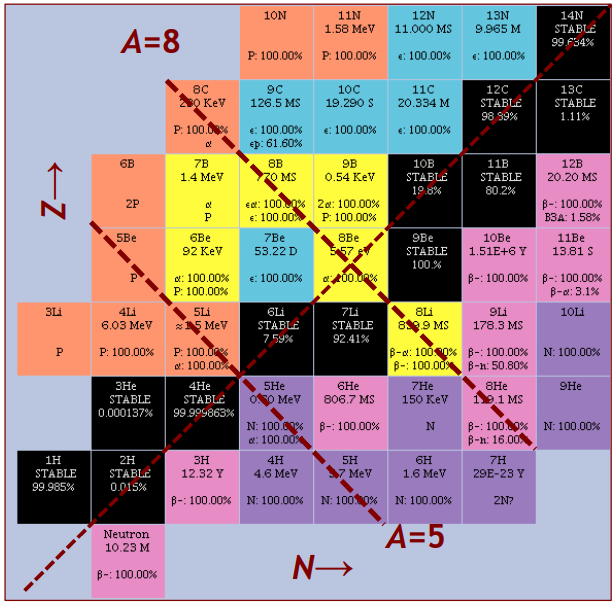
\includegraphics[scale=0.5]{Lezione2/isomeri.png} 
\end{figure}
Abbiamo due definizioni da dare:
\begin{itemize}
    \item \textbf{energia di separazione} è l'energia minima necessaria da fornire ad un nucleone per estrarlo dal nucleo.
\end{itemize}
Per protoni:
\begin{equation*}
    S_p(\ch{^A_Z X})=m(\ch{^{A-1}_{Z-1}X})+m(\ch{^1 H})-m(\ch{^A_Z X})
\end{equation*}
Per neutroni:
\begin{equation*}
    S_n(\ch{^A_Z X})=m(\ch{^{A-1}_{Z}X})+m_n-m(\ch{^A_Z X})
\end{equation*}
Quello che si vede è che $S_p(\ch{^5Li})$ e $S_n(\ch{^5He})$ sono negative. Questo significa che non riesco a prendere un nucleo di elio-4 ed aggiungerci un protone o un neutrone perchè per fare questo al posto di rilasciare energia deve assorbire energia. Questo è il motivo per cui non abbiamo nuclei stabili con $A=5$ perchè parlando di "convenienza energetica" quello che conviene al nucleo di $A=5$ è quello di emettere un protone o un neutrone per diventare elio-4. 

Infine abbiamo che neanche per $A=8$ non esistono nuclei stabili questo perchè se si va a calcolare l'energia di legame di quello che sarebbe il berilio-8 di vede che:
\begin{equation*}
    m(\ch{^8Be})>2m(\ch{^4He})
\end{equation*}
Quindi il berilio-8 quando cerco di formarlo si separa in una situazione energeticamente favorevole dividendosi in due particelle $\alpha$ (accade in frazioni di secondo).
\subsection{Stabilità dei nuclei}
Guardando la carta dei nuclidi si nota che i nuclei stabili si concentrano sulla retta in cui $A=Z$ ma più aumenta il numero di massa più i nuclei stabili si allontanano dalla bisettrice pur mantenendosi in un andamento "lineare". Questa linea è chiamata \textbf{valle di stabilità} e corrisponde ai minimi di energia di legame. Accanto a questi minimi sono presenti due regioni rosa e blu. Queste regioni sono costituite da nuclei instabili che decadono lungo catene di \textbf{isobari} (nuclei con lo stesso $A$, ma diverso $Z$). Quello che abbiamo in queste trasfomazioni tra nuceli isobari: o la trasformazioni di protoni in neutroni ($p\to n$) che corrisponde alla zona blu o il contrario ($n\to p$) che corrisponde alla zona rosa. Queste trasformazioni mi diminuiscono sempre più l'energia (con emissione o cattura di $e$ per conservare la carica) fino a raggiungere l'isobaro più stabile nella valle di stabilità. Questi decadimenti sono classificati in:
\begin{itemize}
    \item $\beta^-$ quando avviene la trasformazione di un neutrone in un protone: $\ch{^A_Z X}\to\ch{^A_{Z+1} X}$ (zona rosa) ($n\to p$).
    \item $\beta^+$ quando avviene la trasformazione di un protone in un neutrone: $\ch{^A_Z X}\to\ch{^A_{Z-1} X}$ (zona blu) ($p\to n$).
\end{itemize}
Come abbiamo detto prima la carica si deve conservare quindi per il decadimento $\beta^-$ viene emesso un elettrone che ha carica elettrica negativa mentre per il decadimento $\beta^+$ viene emesso un positrone che ha carica positiva.

La zona in giallo indica la regione in cui avvengono i decadimenti $\alpha$ sono quelli in cui un atomo decade ed emette un nucleo di elio-4.
\begin{equation*}
    \alpha \quad \ch{^A_Z X}\to\ch{^{A-4}_{Z-2} X}+\ch{^4_2 H}
\end{equation*}
Come abbiamo detto la particella $\alpha$ è uno stato estremamente legato e questo processo permette un guadagno di energia. Le regioni dei decadimenti $\alpha$ è meno estesa e localizzata in nuceli con un $A$ maggiore. 

Ai confini della carta dei nuclidi si possono osservare delle zone viola e delle zone arancioni in cui l'instabilità è tale da far espellere dal nucleo dei neutroni (viola) e dei protoni (arancione). 

Infine, in alto, è presente una parte verde che rappresenta i nuclei in cui è stata riscontrata una fissione spontanea e quindi dove il nucleo si divide in nuclei più piccoli (è molto rara ed avviene solo in nuclei costruiti artificialmente).
\subsection{Modello a goccia}
Cerchiamo di mettere insieme tutte queste informazioni insieme in un modello nucleare. Il primo modello, suggerito da \textbf{Bohr}, che cerca di sistematizzare le osservazioni. Nel seguente modello il nucleo è incompressibile ($R\propto A^{1/3}$), le forze sono a breve range (B.E.$\propto A$) ed è ispirato da una goccia liquida tenuta insieme dalle forze inter-molecolari. Questo modello descrive l'andamento generale dell'energia di legame ma necessita dell'introduzione di termini fenomenologici per descrivere alcune caratteristiche osservate. Questo modello è descritto dalla formula di Bethe-Weizs\"acker (spoiler):
\begin{equation*}
    \text{B.E.}(A,Z)=-a_{1}A+a_{2}A^{\frac{2}{3}}+a_{3}{\frac {Z^2}{A^{\frac{1}{3}}}}+a_{4}{\frac {(N-Z)^{2}}{A}}\pm a_5 A^{-\frac{3}{4}}
\end{equation*}
\subsection{La formula di Bethe-Weizs\"acker}
I primi due termini sono esattamente quelli che ci aspettiamo per una goccia di liquido:
\begin{equation*}
    \text{B.E.}(A,Z)=-a_{1}A+a_{2}A^{\frac{2}{3}}
\end{equation*}
Infatti \textbf{il primo termine} rappresenta l'energia dovuta all'interazione a \textbf{corto range} tra nucleoni vicini. Questo viene dal fatto che nel grafico dell'energia per nucleone dopo una certa $A$ è circa costante. Si può anche tradurre per il fatto che è proporzionale al volume. \textbf{Il secondo termine} è \textbf{positivo} e rappresenta la correzione al primo infatti diminuisce l'energia di legame. Si nota subito come è proporzionale alla superficie del nucleo questo perchè noi sappiamo che il raggio nucleare è proporzionale a $\sim A^{1/3}$ e quindi il termine $A^{2/3}$ risulta proporzionale alla superficie. La motivazione di questo termine deriva dal fatto che i nucleoni interni hanno altri nucleoni vicini in tutte le direzioni. Invece, i nucleoni sulla superficie interagiscono solo con quelli interni (quindi c'è un numero inferiore di interazione e quindi c'è una forza di legame minore rispetto ai nucleoni più interni). \textbf{La correzione all'energia di legame media è più rilevante per nuclei leggeri e spiega l'aumento di B/A per basse masse}. A masse piccole l'energia di legame per nucleone aumenta molto rapidamente.
\begin{equation*}
    a_1=15.753\,MeV \qquad a_2=17.804\,MeV
\end{equation*}
Essendo $A>0$ e con questi valori di $a_1$ e $a_2$ si può facilmente verificare che effettivamente la quantità "correttiva" portato dal secondo termine è minore rispetto alla quantità portata dal primo termine.

Dal punto di vista classico abbiamo sicuramente bisogno di un'altra forza che entra nella struttura nucleare, infatti \textbf{il terzo termine} è la \textbf{repulsione elettrostatica}.
\begin{equation*}
    \text{B.E.}(A,Z)=-a_{1}A+a_{2}A^{\frac{2}{3}}+a_{3}{\frac {Z^2}{A^{\frac{1}{3}}}}
\end{equation*}
Infatti è inversamente proporzionale al raggio del nucleo (dovuto al fatto che l'energia elettrostatica è inversamente proporzionale alla distanza). Ma è anche proporzionale a $Z^2$ (energia elettrostatica direttamente proporzionale al prodotto delle cariche). Questo è un termine che aumenta all'aumentare della massa, per alti valori di $A$ favorisce l'eccesso dei neutroni sui protoni. Questo termine è responsabile alla decrescita di $B/A$ per i nuclei con grande numero atomico. Ad alto $A$ i nuclei hanno anche uno $Z$ grande e il termine di repulsione coulombiana diventa più importante. Quindi questo porta anche al fatto che la curva della valle di stabilità devia dalla bisettrice. Inizialmente i nuclei tendono a favorire un numero uguale di neutroni e protoni ma ad un certo punto deviano da questa situazione che è puro effetto del termine coulombiano. Per calcolare l'ordine di grandezza, infatti l'energia potenziale di una sfera carica uniformemente (oviamente è una approssimazione):
\begin{equation*}
    E=\frac{3}{5}\frac{(Ze)^2}{4\pi\varepsilon_0 R}=\frac{3}{5}\frac{(Ze)^2}{4\pi\varepsilon_0 r_0A^{1/3}}=\frac{3}{5}\frac{(e)^2}{4\pi\varepsilon_0 r_0}\frac{Z^2}{A^{1/3}}=\frac{3}{5}\alpha\frac{\hbar c}{r_0}\frac{Z^2}{A^{1/3}}
\end{equation*}
e quindi, confrontando con il termine dell'equazione di Bethe-Weizs\"acker trovo che:
\begin{equation*}
    a_3\approx\frac{3}{5}\alpha\frac{\hbar c}{r_0} \approx 0.73\,MeV \text{ più precisamente } a_3=0.7103\,MeV
\end{equation*}
Fino a qui è meccanica classica, ma mancano due termini aggiuntivi che non possiamo giustificare senza la meccanica quantistica ottenendo così la formula finale:
\begin{equation*}
    \text{B.E.}(A,Z)=-a_{1}A+a_{2}A^{\frac{2}{3}}+a_{3}{\frac {Z^2}{A^{\frac{1}{3}}}}+a_{4}{\frac {(N-Z)^{2}}{A}}\pm a_5 A^{-\frac{3}{4}}
\end{equation*}
\textbf{Il quarto termine} tiene conto del fatto che i nuclei sono più stabili quando c'è \textbf{simmetria fra protoni e neutroni}: $N\sim Z$, descrive la valle di stabilità. Il termine coulombiano ci potrebbe far pensare di creare dei nuclei con solo neutroni così da raggiungere una situazione di energia favorevole in quanto non presente la repulsione ettrostatica. Ma questo quarto termine ci forza ad avere un numero di protoni circa uguale al numero di neutroni. Per $Z$ piccoli questo è un termine dominante in quanto $N=Z$. Quando vado a cariche grandi c'è una competizione tra questo termine e quello coulombiano (inizia a diventare importante la forza repulsiva che si crea tra i protoni) e questo mi descrive il fatto che la valle di stabilità non è lungo la bisettrice ma deviata.
\textbf{Il quinto termine} descrive una sorta di \textbf{pairing} dei nucleoni cioè che i nuclei sono più stabili se posso formare delle coppie di nucleoni e cioè se posso mettere insieme due protoni o due neutroni insieme. Infatti questo termine è \textbf{nullo} per $A$ dispari, è \textbf{negativo} quando $N$ e $Z$ sono pari (nuclei pari-pari) e \textbf{positivo} quando $N$ e $Z$ sono dispari (nuclei dispari-dispari). In breve se non ci sono nucleoni da soli (non accoppiati con un gemello) i nuclei sono più stabili. Viceversa se nel nucleo è presente un protone o un neutrone da solo il nucleo è meno stabile.
\begin{equation*}
    a_4=23.69\,MeV \qquad a_5=33.6\,MeV
\end{equation*}
Vedremo che il quarto termine è collegato alla struttura quantizzata dei livelli di energia ed al \textbf{Principio di Esclusione di Pauli} mentre il quinto termine esite a causa dell'interazione tra i momenti angolare dei nucleoni.
\subsection{La valle di stabilità B}
La formula dell'energia di legame presenta una evidente regioni di stabilità (stabilità B). Per un dato valore di $A$ l'energia di legame è una parabola al variare di $Z$ in quanto la dipendenza di $Z$ è effettivamente una dipendenza parabolica:
%IMMAGINE rr yy
\begin{figure}[htp!]
  \centering
  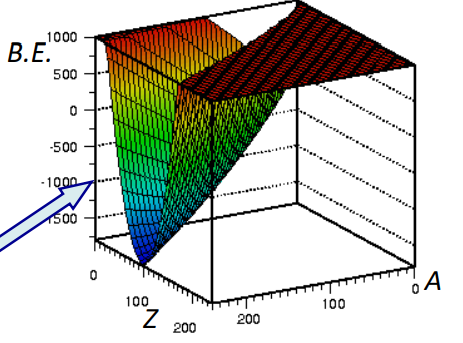
\includegraphics[scale=0.4]{Lezione2/rr.png}
  
\includegraphics[scale=0.4]{Lezione2/yy.png} 
\end{figure}
il primo rappesenta l'energia di legame in funzione di $Z$ e di $A$. Si vede la zona che rappresenta il minimo. Il punto di minimo si trova semplicemente:
\begin{equation*}
    \frac{\partial\text{B.E.}(A,Z)}{\partial Z}\bigg|_{A=\text{cost}}=2a_3\frac{Z}{A^{\frac{1}{3}}}-4a_4\frac{A-2Z}{A}=0
\end{equation*}
\begin{equation*}
    Z=\frac{2a_4A}{a_3A^{\frac{2}{3}}+4a_4}
\end{equation*}
La formula ha i due valori limite:
\begin{equation*}
    Z\to\begin{cases} A/2, & \mbox{piccoli }A \\ \frac{2a_4}{a_3}A^{\frac{1}{3}} & \mbox{grandi }A
\end{cases}
\end{equation*}
Da qui si vede in maniera molto più chiara come per $A$ piccoli $Z$ è praticamente una grandezza in funzione di $A$ mentre per $A$ grandi la retta inizia a piegarsi.
